% Options for packages loaded elsewhere
\PassOptionsToPackage{unicode}{hyperref}
\PassOptionsToPackage{hyphens}{url}
%
\documentclass[
]{book}
\usepackage{amsmath,amssymb}
\usepackage{iftex}
\ifPDFTeX
  \usepackage[T1]{fontenc}
  \usepackage[utf8]{inputenc}
  \usepackage{textcomp} % provide euro and other symbols
\else % if luatex or xetex
  \usepackage{unicode-math} % this also loads fontspec
  \defaultfontfeatures{Scale=MatchLowercase}
  \defaultfontfeatures[\rmfamily]{Ligatures=TeX,Scale=1}
\fi
\usepackage{lmodern}
\ifPDFTeX\else
  % xetex/luatex font selection
\fi
% Use upquote if available, for straight quotes in verbatim environments
\IfFileExists{upquote.sty}{\usepackage{upquote}}{}
\IfFileExists{microtype.sty}{% use microtype if available
  \usepackage[]{microtype}
  \UseMicrotypeSet[protrusion]{basicmath} % disable protrusion for tt fonts
}{}
\makeatletter
\@ifundefined{KOMAClassName}{% if non-KOMA class
  \IfFileExists{parskip.sty}{%
    \usepackage{parskip}
  }{% else
    \setlength{\parindent}{0pt}
    \setlength{\parskip}{6pt plus 2pt minus 1pt}}
}{% if KOMA class
  \KOMAoptions{parskip=half}}
\makeatother
\usepackage{xcolor}
\usepackage{longtable,booktabs,array}
\usepackage{calc} % for calculating minipage widths
% Correct order of tables after \paragraph or \subparagraph
\usepackage{etoolbox}
\makeatletter
\patchcmd\longtable{\par}{\if@noskipsec\mbox{}\fi\par}{}{}
\makeatother
% Allow footnotes in longtable head/foot
\IfFileExists{footnotehyper.sty}{\usepackage{footnotehyper}}{\usepackage{footnote}}
\makesavenoteenv{longtable}
\usepackage{graphicx}
\makeatletter
\def\maxwidth{\ifdim\Gin@nat@width>\linewidth\linewidth\else\Gin@nat@width\fi}
\def\maxheight{\ifdim\Gin@nat@height>\textheight\textheight\else\Gin@nat@height\fi}
\makeatother
% Scale images if necessary, so that they will not overflow the page
% margins by default, and it is still possible to overwrite the defaults
% using explicit options in \includegraphics[width, height, ...]{}
\setkeys{Gin}{width=\maxwidth,height=\maxheight,keepaspectratio}
% Set default figure placement to htbp
\makeatletter
\def\fps@figure{htbp}
\makeatother
\setlength{\emergencystretch}{3em} % prevent overfull lines
\providecommand{\tightlist}{%
  \setlength{\itemsep}{0pt}\setlength{\parskip}{0pt}}
\setcounter{secnumdepth}{5}
\usepackage{booktabs}
\ifLuaTeX
  \usepackage{selnolig}  % disable illegal ligatures
\fi
\usepackage[]{natbib}
\bibliographystyle{plainnat}
\IfFileExists{bookmark.sty}{\usepackage{bookmark}}{\usepackage{hyperref}}
\IfFileExists{xurl.sty}{\usepackage{xurl}}{} % add URL line breaks if available
\urlstyle{same}
\hypersetup{
  pdftitle={Manifolds},
  pdfauthor={Ashan Jayamal \& Nalamudu Samarasinghe},
  hidelinks,
  pdfcreator={LaTeX via pandoc}}

\title{Manifolds}
\author{Ashan Jayamal \& Nalamudu Samarasinghe}
\date{2024-03-10}

\usepackage{amsthm}
\newtheorem{theorem}{Theorem}[chapter]
\newtheorem{lemma}{Lemma}[chapter]
\newtheorem{corollary}{Corollary}[chapter]
\newtheorem{proposition}{Proposition}[chapter]
\newtheorem{conjecture}{Conjecture}[chapter]
\theoremstyle{definition}
\newtheorem{definition}{Definition}[chapter]
\theoremstyle{definition}
\newtheorem{example}{Example}[chapter]
\theoremstyle{definition}
\newtheorem{exercise}{Exercise}[chapter]
\theoremstyle{definition}
\newtheorem{hypothesis}{Hypothesis}[chapter]
\theoremstyle{remark}
\newtheorem*{remark}{Remark}
\newtheorem*{solution}{Solution}
\begin{document}
\maketitle

{
\setcounter{tocdepth}{1}
\tableofcontents
}
\hypertarget{basic-theroms-and-definitions}{%
\chapter{Basic Theroms and Definitions}\label{basic-theroms-and-definitions}}

\begin{definition}[Topology]
\protect\hypertarget{def:Top}{}\label{def:Top}A topology on a set \(X\) is a collection \(\mathcal{T}\) of subsets of \(X\) such that

\textbf{(T1)} \(\phi\) and \(X\) are in \(\mathcal{T}\);

\textbf{(T2)} Any union of subsets in \(\mathcal{T}\) is in \(\mathcal{T}\);

\textbf{(T3)} The finite intersection of subsets in \(\mathcal{T}\) is in \(\mathcal{T}\).
\end{definition}

A set \(X\) with a topology \(\mathcal{T}\) is called a topological space. Denoted by \((X,\mathcal{T})\). An element of \(\mathcal{T}\) is called an open set.

\begin{definition}
\protect\hypertarget{def:unnamed-chunk-1}{}\label{def:unnamed-chunk-1}A subset \(U \subset M\) is referred to as open in \(M\) if \(U \in \mathcal{T}\). A subset \(A \subset M\) is termed closed if \(M \setminus A \in \mathcal{T}\).
\end{definition}

\begin{definition}[Continuity]
\protect\hypertarget{def:unnamed-chunk-2}{}\label{def:unnamed-chunk-2}If both \((M, \mathcal{T}_M)\) and \((N, \mathcal{T}_N)\) are topological spaces, a map \(f : M \rightarrow N\) is termed continuous if \[f^{-1}(V) \in \mathcal{T}_M \text{ for all } V \in \mathcal{T}_N\].
In other words, the preimages of open sets must be open.
\end{definition}

\begin{definition}[Homemorphism]
\protect\hypertarget{def:unnamed-chunk-3}{}\label{def:unnamed-chunk-3}A map \(f : M \rightarrow N\) between two topological spaces is called homemorphism if it has following propoties.
- \(f\) is a bijection,
- \(f\) is continuous,
- the inverse function \(f^{-1}\) is continuous.

Two topological spaces \(M\) and \(N\) are called homeomorphic if there exists a homeomorphism between them.
\end{definition}

\begin{definition}[Hausdorff Space]
\protect\hypertarget{def:unnamed-chunk-4}{}\label{def:unnamed-chunk-4}A topological space \((X,\mathcal{T})\) is called a Hausdorff space if\\
\textbf{(H1)} \(\forall x,y \in X\) such that \(x \neq y\), \(\exists U_x, U_y \in \mathcal{T}\) such that \(x \in U_x\), \(y \in U_y\), and \(U_x \cap U_y = \emptyset\).

i.e., for every pair of distinct points \(x, y\) in \(X\), there are disjoint neighborhoods \(U_x\) and \(U_y\) of \(x\) and \(y\) respectively.
\end{definition}

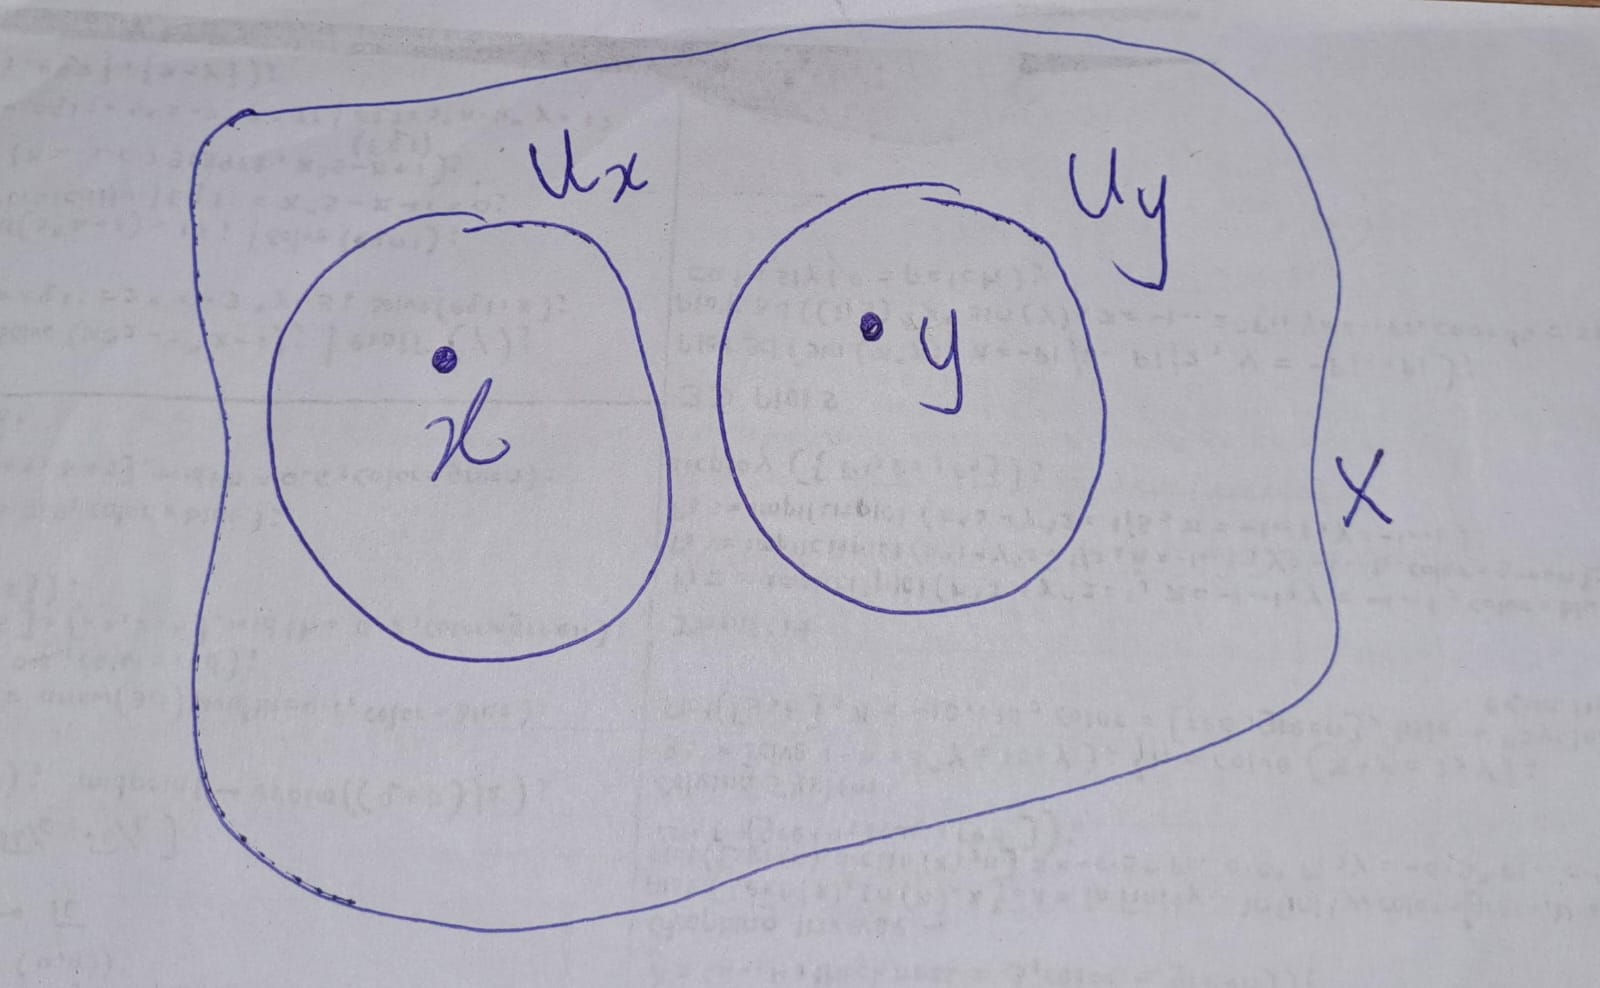
\includegraphics{figures/ch1/fig01.jpg}
::: \{.definition \#unnamed-chunk-5 name=``Countability''\}
A space \(X\) is said to have a \textbf{countable basis at the point \(x\)} if there is a countable collection \(\{U_n\}_{n\in\mathbb{Z}^+}\) of neighborhoods of \(x\) such that any neighborhood \(U\) of \(x\) contains at least one of the sets \(U_n\). A space \(X\) that has a countable basis at each of its points is said to satisfy the first countability axiom.
:::

\hypertarget{stereographic-projection}{%
\subsection{Stereographic Projection}\label{stereographic-projection}}

\begin{itemize}
\tightlist
\item
  \textbf{Stereographic Projection plane \(\mathbb{R}\) and the 1-sphere minus a point}\\
  The 1-sphere \(S^1\) is the set of points \((x,y,z) \in \mathbb{R}^3\) such that \(x^2 + y^2 + z^2 = 1\).
  \[S^1:=\{(x,y): ||(x,y)||=1\}\]
\end{itemize}

Let \(S^1 \setminus \{N\}\) denote the 1-sphere minus (circle) its north pole, i.e., the point \((0,1)\).

There exists a homeomorphism \(\varphi : S^1 \setminus \{N\} \to \mathbb{R}\), which can be described as follows. In coordinates, this map is precisely
\[\varphi(x,y) = \frac{x}{1-y}\]

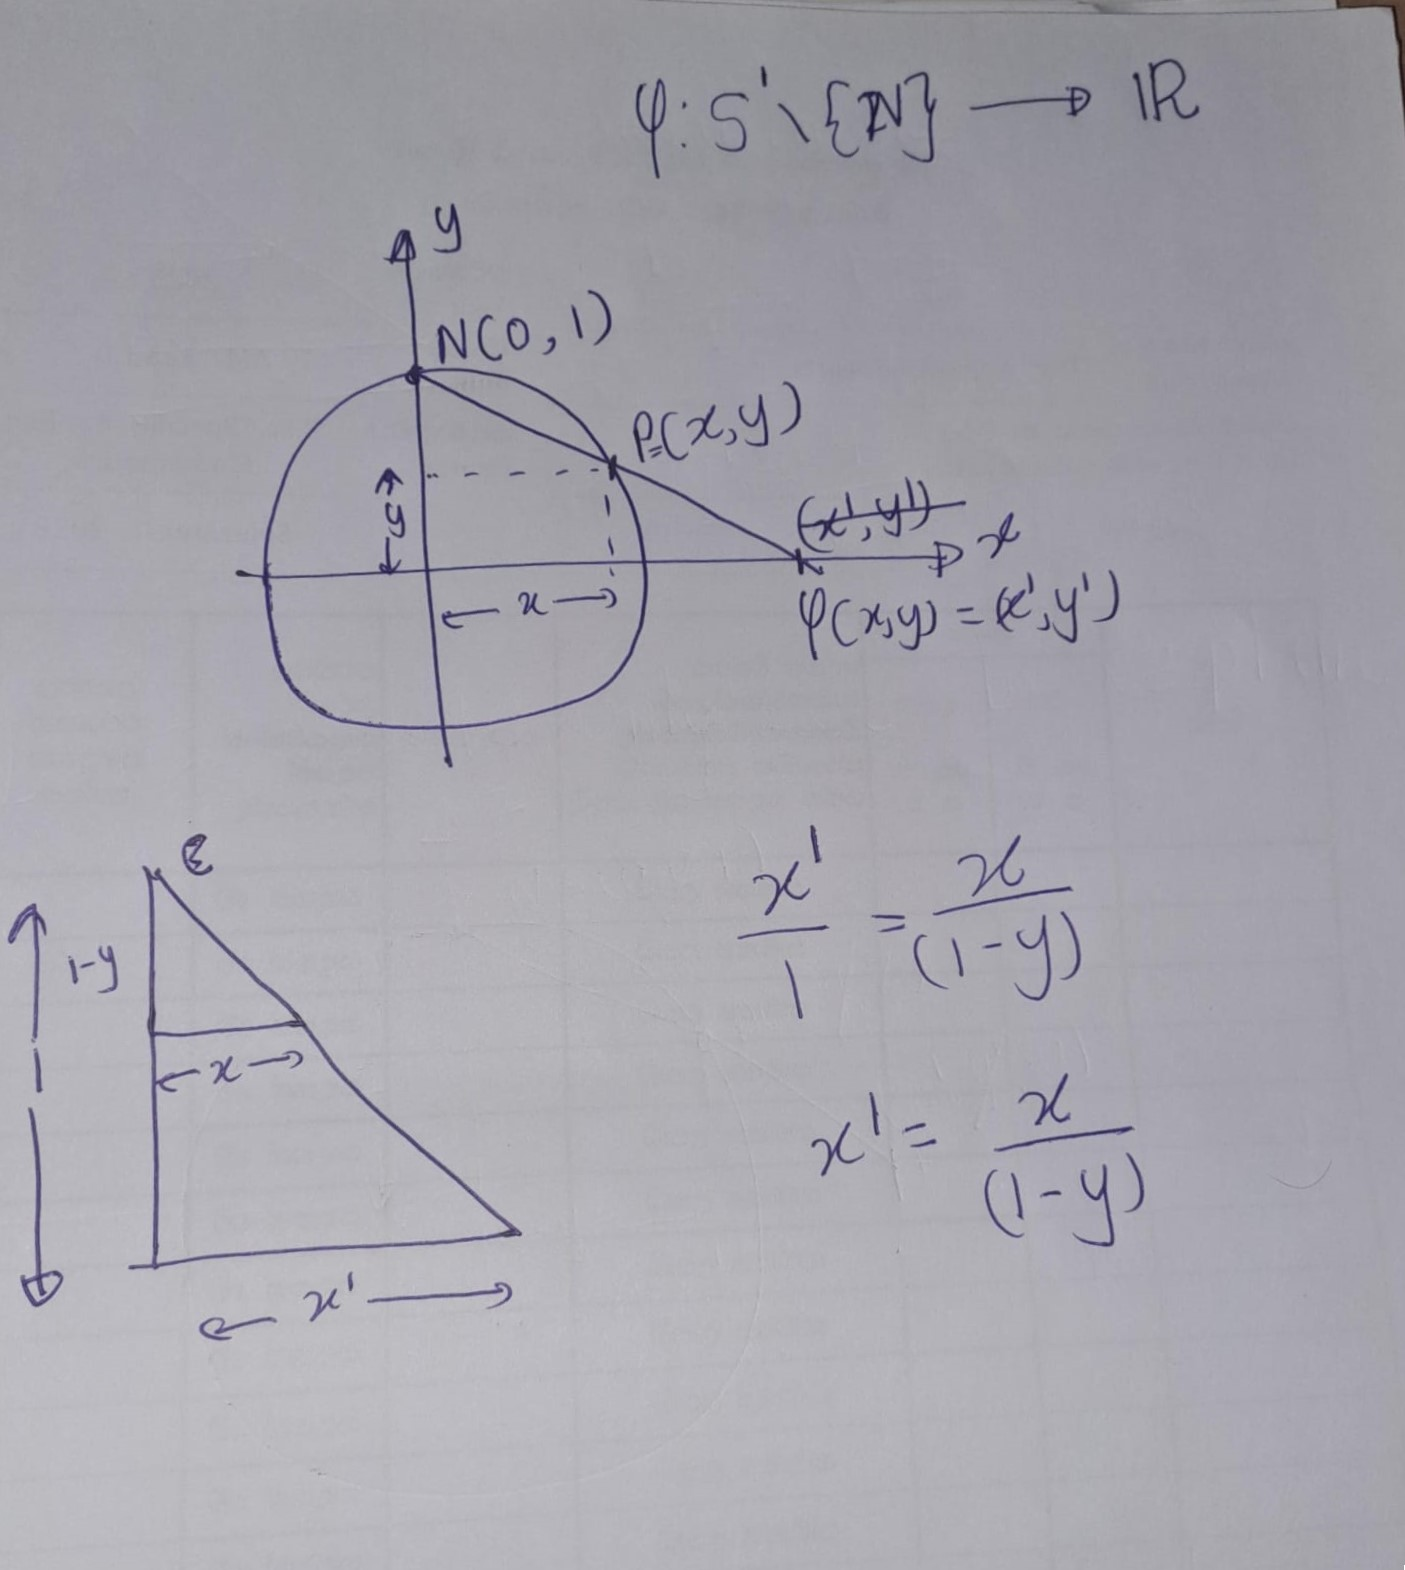
\includegraphics{figures/ch1/fig05.jpg}
- \textbf{Stereographic Projection plane \(\mathbb{R}^2\) and the 2-sphere minus a point}\\

Stereographic projection is an important homeomorphism between the plane \(\mathbb{R}^2\) and the 2-sphere minus a point. The 2-sphere \(S^2\) is the set of points \((x,y,z) \in \mathbb{R}^3\) such that \(x^2 + y^2 + z^2 = 1\). Let \(S^2 \setminus \{N\}\) denote the 2-sphere minus its north pole, i.e., the point \((0,0,1)\).

There exists a homeomorphism \(\varphi : S^2 \setminus \{N\} \to \mathbb{R}^2\), which can be described as follows.

For a point \(p \in S^2 \setminus \{N\}\), let \(\varphi(p)\) denote the unique point in \(P\) such that the intersection of the segment \(\overline{Nf(p)}\) and \(S^2\) is \(p\). In coordinates, this map is precisely
\[\varphi(x,y,z) = \left(\frac{x}{1-z}, \frac{y}{1-z}\right).\]

\begin{figure}
\centering
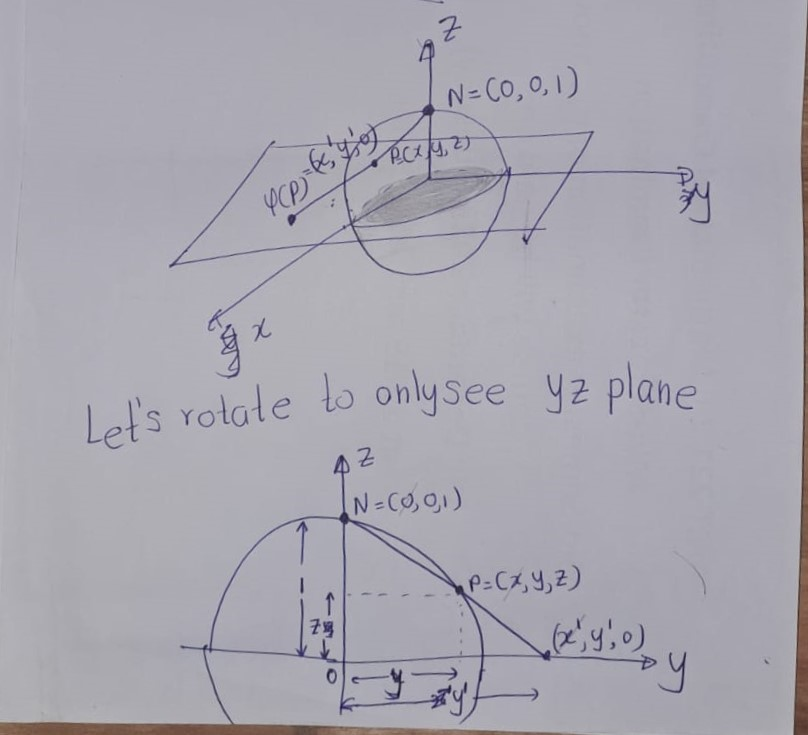
\includegraphics{figures/ch1/fig03.jpg}
\caption{\label{fig:fig03}\(~\)}
\end{figure}

\begin{figure}
\centering
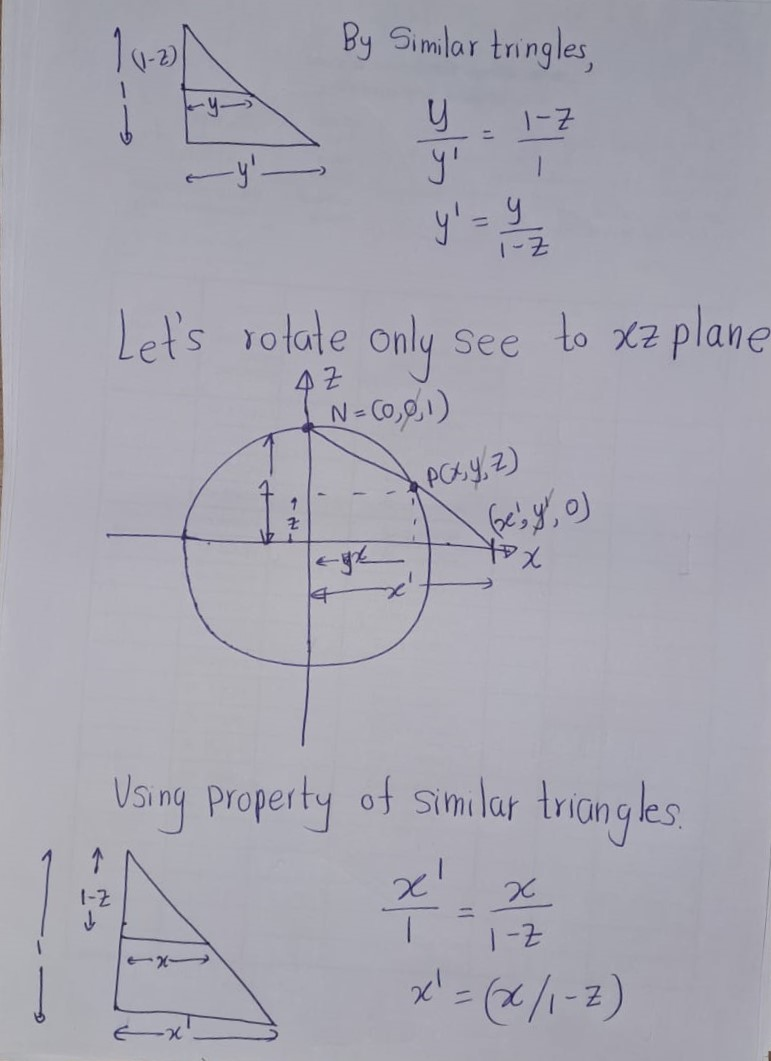
\includegraphics{figures/ch1/fig04.jpg}
\caption{\label{fig:fig04}\(~\)}
\end{figure}

\begin{definition}
\protect\hypertarget{def:unnamed-chunk-6}{}\label{def:unnamed-chunk-6}If \(X\) is a space, a point \(x\) of \(X\) is said to be an \textbf{isolated point} of \(X\) if the one-point set \(\{x\}\) is open in \(X\).
\end{definition}

\hypertarget{manifolds}{%
\chapter{Manifolds}\label{manifolds}}

\hypertarget{topological-manifolds}{%
\section{Topological Manifolds}\label{topological-manifolds}}

\begin{definition}
\protect\hypertarget{def:topmanifold}{}\label{def:topmanifold}

Let \((M,\mathcal{T})\) be a topological space with topology \(\mathcal{T}\). Then \(M\) is called an \(n\)-dimensional topological manifold, if the following holds:

\begin{itemize}
\tightlist
\item
  \textbf{(TM1)}: \(M\) is Hausdorff.
\item
  \textbf{(TM2)}: The topology of \(M\) has a countable basis.
\item
  \textbf{(TM3)}: \(M\) is locally homeomorphic to \(\mathbb{R}^n\), that is, for all \(p \in M\) exists an open subset \(U \subset M\) with \(p \in U\), an open subset \(V \subset \mathbb{R}^n\) and a homeomorphism \(\varphi : U \rightarrow V\).
\end{itemize}

\end{definition}

\begin{figure}
\centering
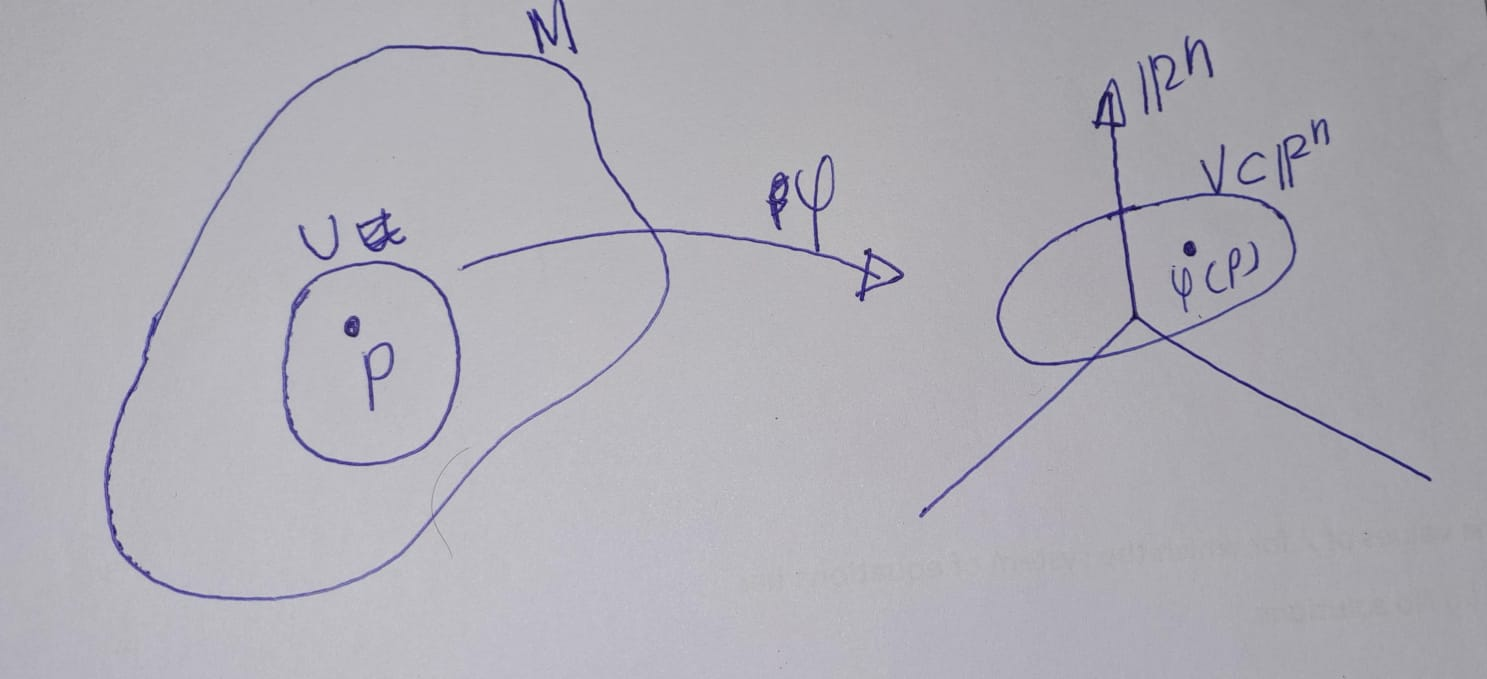
\includegraphics{figures/ch1/fig02.jpg}
\caption{\label{fig:fig02}\(~\)}
\end{figure}

\begin{remark}
The first two conditions in the definition \ref{def:topmanifold} are more of a technical nature and are sometimes neglected. The important fact is that a topological manifold is locally homeomorphic to \(\mathbb{R}^n\). Loosely speaking, manifolds look locally like Euclidean space. If the topology on \(M\) is induced by a metric, then the first condition is satisfied automatically. If \(M\) is given as a subset of \(\mathbb{R}^N\) with the subset topology, then both conditions M1 and M2 are satisfied automatically.
\end{remark}

Let's see some examples.

\begin{example}
\protect\hypertarget{exm:unnamed-chunk-8}{}\label{exm:unnamed-chunk-8}

Euclidean space \(M=\mathbb{R}^n\) itself is an \(n\)-dimensional topological manifold:

\begin{itemize}
\tightlist
\item
  (TM1): We know that \(\mathbb{R}^n\) is metrc space. Let's say the metric as \(d\). Let \(x,y\in \mathbb{R}^n\) with \(x\neq y\).
  Let \(r=d(x,y)\). Since \(x\neq y\),\(r>0\).
  Let \(U_x=B(x,r/2)\) and \(U_y=B(y,r/2)\).
  So, \(x\in U_x\) and \(y\in U_y\) We need to show that \(U_x \cap U_y\neq \emptyset\). We are going to proof by contrdiction. So, asssume the contray, there exist \(z\in U_x\cap U_y\). Thus,
  \(d(x,z)<r/2\) and \(d(y,z)<r/2\). Then,
  \[r=d(x,y)\leq d(x,z)+d(z,y)=d(x,z)+d(y,z)<\frac{r}{2}+\frac{r}{2}=r\]
  This is contradiction. Hence \(U_x\cap U_y \neq \emptyset\). Therefore \(M=\mathbb{R}^n\) is Hausdorff.
\item
  (TM2): Later I will update this part
\end{itemize}

{Problem \textbf{:(}}.

\begin{itemize}
\tightlist
\item
  (TM3): Let \(U=\mathbb{R}^n=M\) and \(V=\mathbb{R}^n\) and \(\varphi=id\). We can easily tell that idenntity map is bijective. Furthur, we can observe that inverse of identity map is itself and it is well defined.
  So, Let \(U'\subset U=\mathbb{R}^n\) be an open set
  \[\forall x\in U'\quad id^{-1}(x)=id(x)=x\]. Thus, \[id(U')=id^{-1}(U')=U'.\] Hence, by definition of continuous mapping, \(id\) and \(id^{-}\) are continuous.
\end{itemize}

\end{example}

\begin{example}
\protect\hypertarget{exm:unnamed-chunk-9}{}\label{exm:unnamed-chunk-9}Let \(M \subset \mathbb{R}^n\) be an open subset. Then \(M\) is an \(n\)-dimensional topological manifold.\\
(TM1), (TM2) Obvious.\\
(TM3) Holds true with \(U = M\), \(V = M\) and \(x = \text{id}\).

Here Ia m not going to proove this. It is very similar to first example.
\end{example}

\begin{example}
\protect\hypertarget{exm:unnamed-chunk-10}{}\label{exm:unnamed-chunk-10}The standard sphere \(M = S^n = \{ \underline{y}=(y^0,...,y^{n}) \in \mathbb{R}^{n+1} : ||\underline{y}|| = 1 \}\) is an \(n\)-dimensional topological manifold.

\begin{itemize}
\tightlist
\item
  (TM1) and (TM2) , since \(S^n\) is a subset of \(\mathbb{R}^{n+1}\).
\item
  (TM3) We construct two homeomorphisms with the help of the stereographic projection. Let \(N\) be north pole of the n-sphere, that is \((\underbrace{0,...,0}_{n~times},1)\in \mathbb{R}^{n+1}\). Let \(U_1:=S^n\setminus \{N\}\) and \(v_1=\mathbb{R}^{n+1}\). We define
\end{itemize}

\begin{eqnarray}
\varphi:U_1&\to & V_1\\
\underline{y} =(y^0,y^1,...,y^n) & \mapsto & \frac{(y^0,y^1,...,y^n)}{1-y^{n+1}}
\end{eqnarray}
- Cliam 1: \(varphi\) is injective.\\
Let \((x^0,...,x^{n}),(y^0,y^1,...,y^n)\in \mathbb{R}^n\). Suppose that \(\varphi(x^0,...,x^{n})=\varphi(y^0,y^1,...,y^n)\).
\begin{eqnarray}
\varphi(x^0,...,x^{n})&=&\varphi(y^0,y^1,...,y^n)\\
\frac{(x^0,x^1,...,x^n)}{1-x^{n+1}}&=&\frac{(y^0,y^1,...,y^n)}{1-y^{n+1}}\\
(y^0, y^1, ..., y^n)(1-x^{n+1}) &=& (x^0, x^1, ..., x^n)(1-y^{n+1})\\
(y^0 - y^0x^{n+1}, y^1 - y^1x^{n+1}, ..., y^n - y^nx^{n+1}) &=& (x^0 - x^0y^{n+1}, x^1 - x^1y^{n+1}, ..., x^n - x^ny^{n+1})\\
y^0(1 - x^{n+1}), y^1(1 - x^{n+1}), ..., y^n (1- y^nx^{n+1}) &=&  x^0(1-y^{n+1}), x^1(1 - y^{n+1}), ..., x^n (1- y^{n+1})\\
\end{eqnarray}
Thus, \(y^i(1 - x^{n+1}) = x^i(1 -y^{n+1})\) for all \(i = 0, 1, ..., n\).
Since \(1 - y^{n+1}, 1 - x^{n+1} > 0\),
?

?

?

?

{Problem HOW INJECTIVITY COMES\textbf{:(}}.

{CHECK\textbf{:(}}.\\
- Claim 2: \(\varphi\) is surejctive.~
Surjectivity means that for every \(\underline{v} \in V_1 = \mathbb{R}^n\), there exists some \(\underline{y} \in U_1\) such that \(\varphi(\underline{y}) = \underline{v}\).

So, let \(\underline{v} = (v^0, v^1, ..., v^n) \in V_1\). We need to find \(\underline{y} = (y^0, y^1, ..., y^n) \in U_1\) such that

\[\frac{(y^0, y^1, ..., y^n)}{1-y^{n+1}} = \underline{v}.\]

We can solve this equation for \(\underline{y}\) as follows:

\[\underline{y} = (1-y^{n+1})\underline{v} = \underline{v} - y^{n+1}\underline{v}.\]

We know that \(\underline{y} \in U_1 = S^n \setminus \{N\}\), so \(y^{n+1} = 1 - \|\underline{y}\|^2\). Substituting this into the equation gives us

\[\underline{y} = \underline{v} - (1 - \|\underline{y}\|^2)\underline{v} = \|\underline{y}\|^2\underline{v}.\]

Solving this equation for \(\|\underline{y}\|^2\) gives us

\[\|\underline{y}\|^2 = \frac{\|\underline{v}\|^2}{1 + \|\underline{v}\|^2}.\]

Substituting this back into the equation for \(\underline{y}\) gives us

\[\underline{y} = \frac{\underline{v}}{1 + \|\underline{v}\|^2}.\]

This is a well-defined point in \(U_1\) for every \(\underline{v} \in V_1\), so \(\varphi\) is surjective.

\begin{itemize}
\tightlist
\item
  Claim: \(\varphi\) is continuous.\\
  Note that the inverse map \(\phi\) is given by,
  \begin{eqnarray}
  \phi : V_1 &\rightarrow & U_1\\
  \underline{x}= (x^0, x^1, ... , x^n) &\mapsto & \frac{(x^0,x^1,...,x^{n-1})}{1 + x^n} 
  \end{eqnarray}
  {I will update this proof. I want some to to write rigirs proof\textbf{:(}}.
\end{itemize}

Analogously, we define the homeomorphism, which omits the south pole:
Let now \(U_2 := S^n \setminus \{S\}\) with \(S := ( 0,... , 0, -1) \in \mathbb{R}^{n+1}\) and \(V_2 := \mathbb{R}^n\).
Then
\begin{eqnarray}
\varphi : U_2 &\rightarrow & V_2,\\
\underline{y}= (y^0, y^1, ... , y^n) &\mapsto & \frac{(y^0,y^1,...,y^n)}{1 + y^n} 
\end{eqnarray}

Therefore, \(n\)-sphere \(S^n\) is an \(n\)-dimensional topological manifold.
\end{example}

\begin{example}[Non-Example]
\protect\hypertarget{exm:unnamed-chunk-11}{}\label{exm:unnamed-chunk-11}We consider \(M := \{ (y^1, y^2, y^3) \in \mathbb{R}^3 | (y^1)^2 = (y^2)^2 + (y^3)^2 \}\), the double cone.

Since \(M \subset \mathbb{R}^3\), both (i) and (ii) are satisfied.

But \(M\) is \textbf{not} a 2-dimensional manifold. Assume it were, then there would exist an open subset \(U \subset M\) with \(0 \in U\), an open subset \(V \subset \mathbb{R}^2\) and a homeomorphism \(\varphi : U \rightarrow V\) with \(\varphi(0) = 0\).
{How do we Gruntee that such hormouphsim exsist that maps 0 to 0\textbf{:(}}
Without losss of generality assume \(V = B_r(x(0))\) with \(r > 0\). Choose \((p^1,p^2,p^3), (q^1,q^2,q^3) \in U\) with \(p^1 > 0\) and \(q^1 < 0\). Furthermore, choose a continuous path \(c : [0, 1] \rightarrow V\) with \(c(0) = x(q_1)\), \(c(1) = x(q_2)\) and \(c(t) \neq x(0)\) for all \(t \in [0, 1]\).

Define the continuous path \(\tilde{c} := x^{-1} \circ c : [0, 1] \rightarrow U\). Then \(\tilde{c}(0) = q_1\), \(\tilde{c}(1) = q_2\), that is, we have \(\tilde{c}_1(0) > 0\) while \(\tilde{c}_1(1) < 0\). Applying the mean value theorem we find, that there exists a \(t \in (0, 1)\) with \(\tilde{c}_1(t) = 0\). Then \(\tilde{c}(t) = (0, 0, 0)\) and consequently \(c(t) = x(\tilde{c}(t)) = x(0)\), which contradicts the choice of \(c\). Hence, \(M\) is not a 2-dimensional topological manifold.
\end{example}

\begin{definition}[charts]
\protect\hypertarget{def:unnamed-chunk-12}{}\label{def:unnamed-chunk-12}If \(M\) is an \(n\)-dimensional topological manifold, the homeomorphisms \(\varphi : U \to V\) are called charts (or local coordinate systems) of \(M\).
\end{definition}

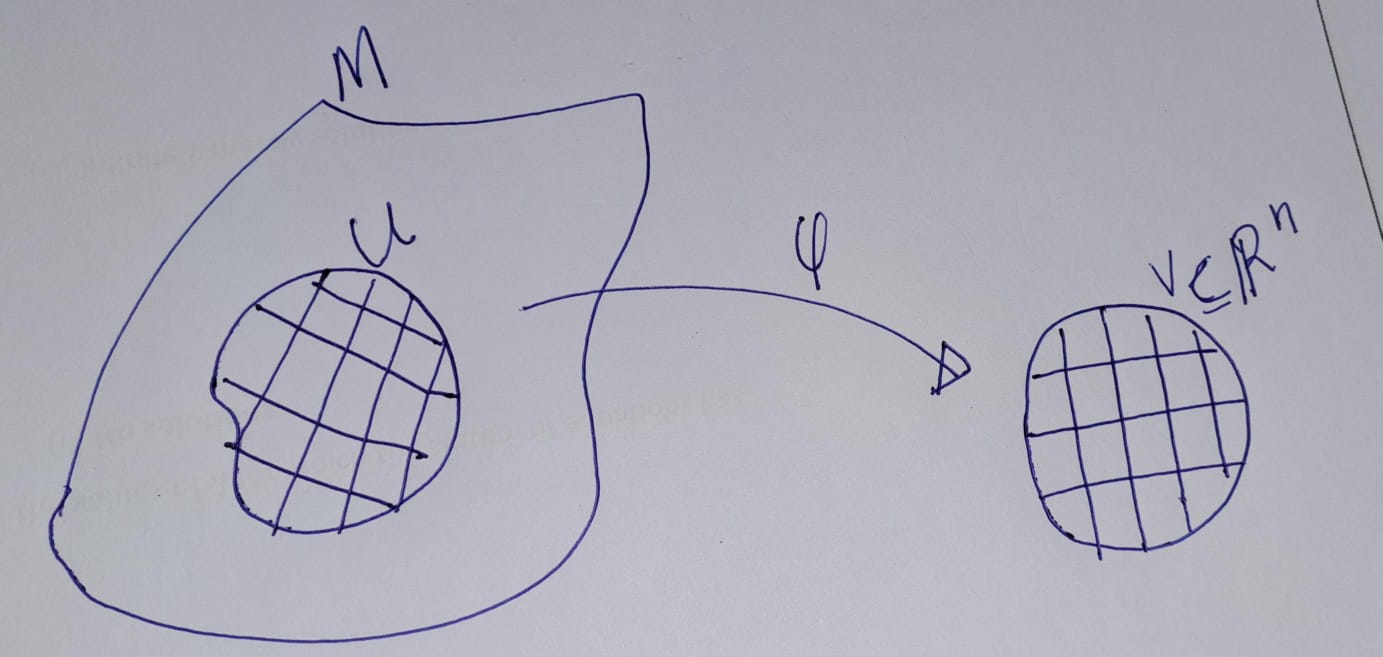
\includegraphics{figures/ch1/fig06.jpg}
After choosing a local coordinate system \(\varphi : U \rightarrow V\) every point \(p \in U\) is uniquely characterized by its coordinates \((\varphi^1(p), \ldots , \varphi^n(p))\).

\begin{example}[0-dimesional manifold]
\protect\hypertarget{exm:unnamed-chunk-13}{}\label{exm:unnamed-chunk-13}In a \(0\)-dimensional manifold \(M\) every point \(p \in M\) has an open neighborhood \(U\), which is homeomorphic to \(R^0 = \{0\}\). Consequently \(\{p\} = U\) is an open subset of \(M\) for all
\(p \in M\), that is, \(M\) carries the discrete topology. Since there exists a countable basis for the topology on \(M\) and the topology is discrete in addition, \(M\) has to be countable itself.
\end{example}

\begin{figure}
\centering
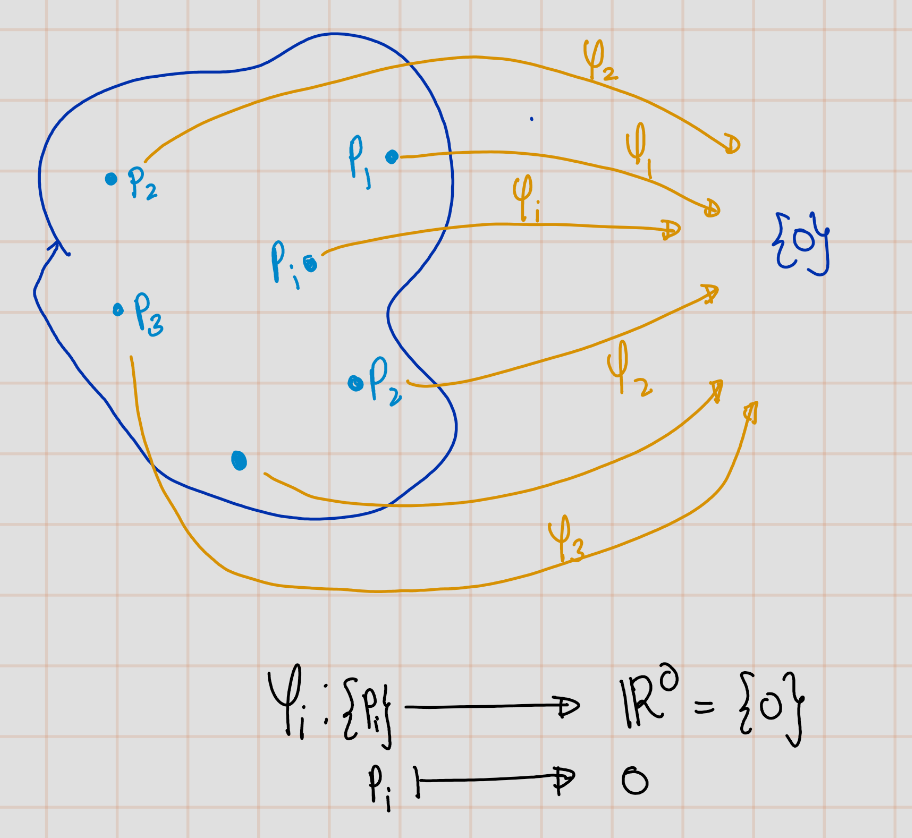
\includegraphics{figures/ch1/fig07.png}
\caption{\label{fig:fig07}\(~\)}
\end{figure}

\begin{proposition}
\protect\hypertarget{prp:unnamed-chunk-14}{}\label{prp:unnamed-chunk-14}A topological space \(M\) is a 0-dimensional topological manifold, if and only if \(M\) is countable and carries the discrete topology.
\end{proposition}

\begin{proof}
\leavevmode

\begin{itemize}
\item
  (\(\implies\)) By definition, a 0-dimensional topological manifold is a topological space where every point has a neighborhood homeomorphic to the 0-dimensional Euclidean space, which is a single point \(\{0\}\). This implies that for every point \(p \in M\), there exists an open neighborhood \(U\) such that \(\{p\} = U\). This is exactly the definition of a discrete topology.

  Since, there exists a countable basis for the topology on \(M\), and every point in \(M\) is an open set (i.e., the topology is discrete), then \(M\) must be countable. This is because every point in \(M\) corresponds to an open set in the basis, and since the basis is countable, \(M\) must also be countable.
\item
  (\(\Longleftarrow\)) If \(M\) carries the discrete topology, then every subset of \(M\) is open. In particular, for every point \(p \in M\), the set \(\{p\}\) is an open set. This means that every point in \(M\) has a neighborhood homeomorphic to the 0-dimensional Euclidean space, which is a single point \(\{0\}\). This is exactly the definition of a 0-dimensional topological manifold.

  If \(M\) is countable, then there exists a countable basis for the topology on \(M\). Since every point in \(M\) is an open set (i.e., the topology is discrete), this basis can be taken to be the set of all singletons \(\{p\}\), where \(p \in M\).
\end{itemize}

Therefore, a topological space \(M\) is a 0-dimensional topological manifold if and only if \(M\) is countable and carries the discrete topology.

\end{proof}

\begin{definition}
\protect\hypertarget{def:unnamed-chunk-16}{}\label{def:unnamed-chunk-16}A topological manifold \(M\) is said to be \textbf{connected}, if for every two points \(p, q \in M\) there exists a continuous map \(c : [0, 1] \to M\) with \(c(0) = p\) and \(c(1) = q\).
\end{definition}

\begin{figure}
\centering
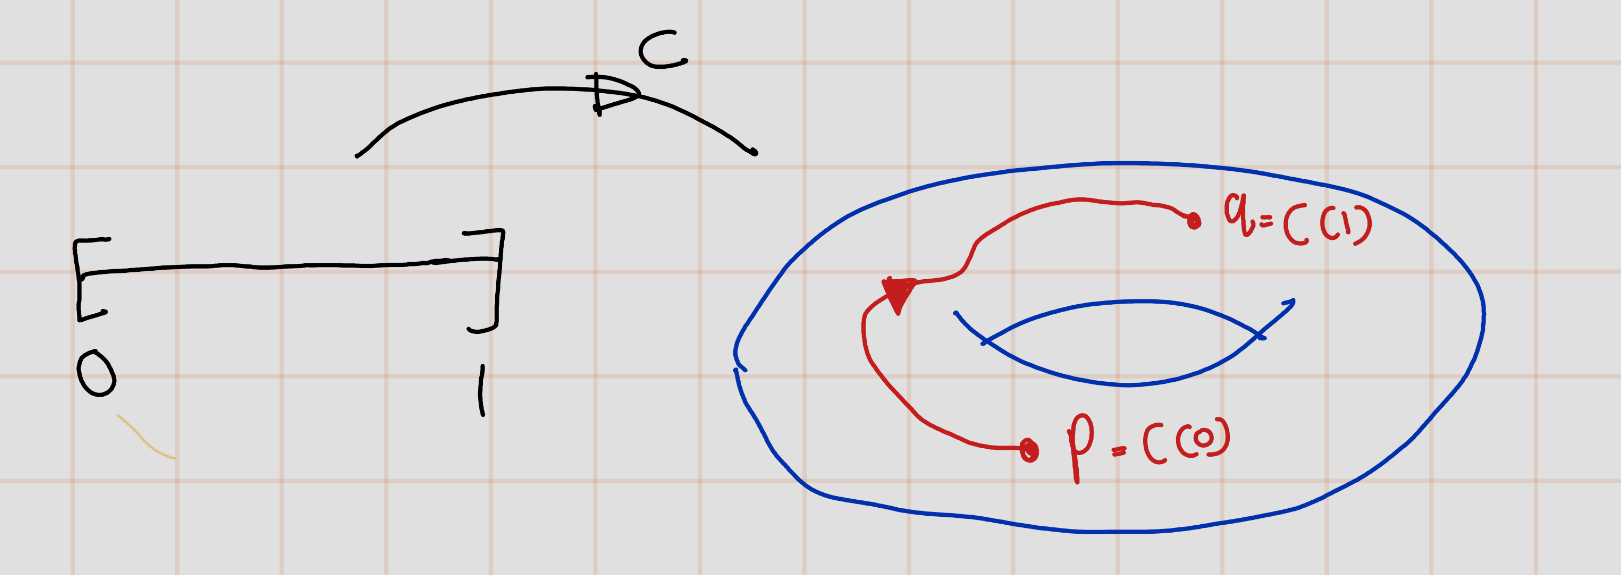
\includegraphics{figures/ch1/fig08.png}
\caption{\label{fig:fig08}\(~\)}
\end{figure}

Given two points, there has to be a continuous curve in \(M\) which connects both. Usually, in Topology one calls this path-connected, which is in the case of manifolds equivalent to being connected. We do not want to go deeper into this subject at this point.

\begin{center}\includegraphics[width=800px,height=460px]{pdf_docs/0DimesionalManifold} \end{center}

  \bibliography{book.bib,packages.bib}

\end{document}
